\documentclass{beamer}

\usepackage[italian]{babel}

\usepackage[utf8]{inputenc}

\newcommand{\R}{\mathbb{R}}
\newcommand{\Z}{\mathbb{Z}}
\newcommand{\mc}[1]{\mathcal{#1}}
\newcommand{\ii}[1]{\textit{#1}}
\newcommand{\req}[1]{\stackrel{#1}{=}}
\newcommand{\bra}[1]{\langle #1 |}
\newcommand{\ket}[1]{| #1 \rangle}
\newcommand{\braket}[2]{\langle #1 | #2 \rangle}

\title{Un'Introduzione Matematica al \\ Geometric Deep Learning}
\author{Tommaso Lamma}
\date{2021}

\begin{document}

\section{Introduzione}

\frame{\titlepage}

\begin{frame}
    \frametitle{Reti Convoluzionali}
    \begin{figure}[H]
        \centering
        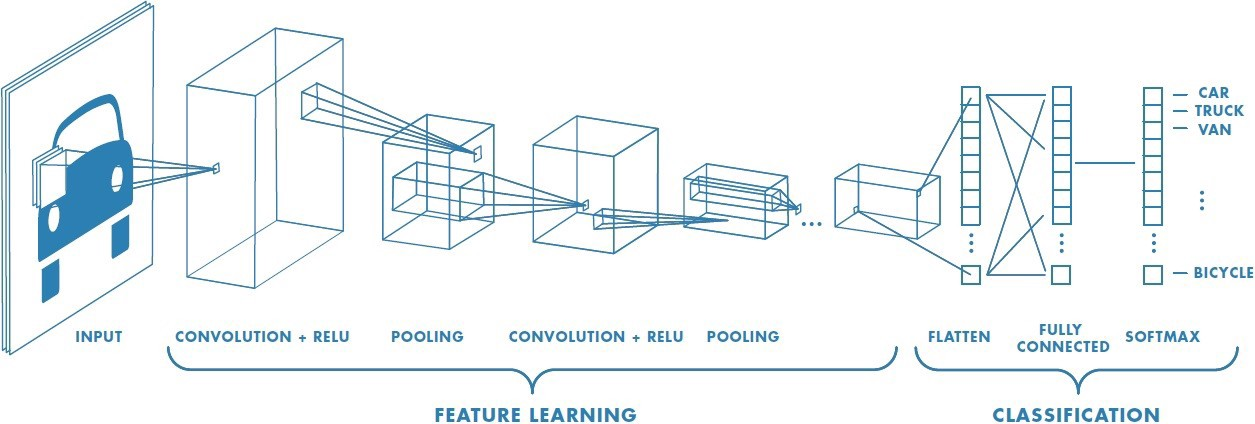
\includegraphics[width=10cm, height=4cm]{cnn}
        \caption{Una rete neurale convoluzionale.}
    \end{figure}       
\end{frame}

\begin{frame}
    \frametitle{Convoluzione su Domini Euclidei}    
    Siano $f:\R^n \to \R$ e $g:\R^n \to \R$,
    \[ (f * g)(x) = \int_{\R^n} dx' f(x')g(x-x'). \]
    \hfill \\
    \hfill \\
    { \large Cosa significa $(x - x')$ in un dominio diverso da $\R^n$ ?}
\end{frame}

\begin{frame}
    \frametitle{ \large Cosa significa $(x - x')$ \textbf{in} $\R^n$ ?}
    \hfill \\
    \hfill \\
    Possiamo vedere $( x - x')$ come l'azione dell'elemento $(-x')$ del gruppo delle traslazioni $(\R^n, +)$
    sul dominio $\R^n$(A priori della struttura di spazio vettoriale).
    \begin{block}{Notare:}
        Il gruppo $(\R^n, +)$ è una simmetria globale del dominio $\R^n$.  
    \end{block}
    \hfill \\
    \hfill \\
    {\large Possiamo definire una convoluzione su un dominio a partire dalla simmetria globale del dominio?}
\end{frame}

\begin{frame}
    \begin{figure}[H]
        \centering
        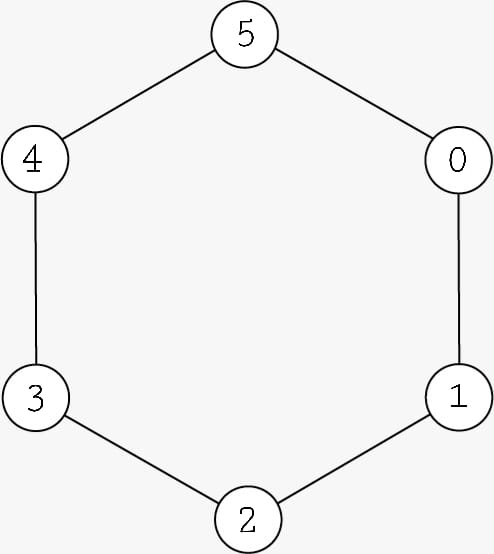
\includegraphics[width=5cm, height=5cm]{graph}
        \caption{}
    \end{figure}    
\end{frame}


\end{document}